% #1 is the caption name, #2 is the caption text
\newcommand{\definecaption}[2]{%
   \expandafter\newcommand\csname caption@#1\endcsname{#2}}

\newcommand{\usecaption}[1]{%
   \caption{\csname caption@#1\endcsname\label{#1}}}

% Now the captions

%_______________________________________________________________
\definecaption{F_scheme}{%
%
Space--time diagrams showing a schematic representation of the
different stages in the development of causal contact node (\ceti{}).
%
Panel (a) represents the region $R$ in space and time which is causally
connected to the emitter (left vertex), following an "A" type event
("Awakening") in which the node acquires the communication capability.
%
The sphere of first contact (SFC) is a sphere centered on the emitter
that grows until its radius reaches the D$_{max}$ distance, in which
the power of a signal would equal the detectability threshold.
%
In the Figure this sphere is represented by the left triangle of the
region $R$.
%
The surface of last contact (SLC) is another sphere that grows from a
"D" event ("Doomsday").
%
The region which is causally connected to the emitter is then limited
by these two spheres, and has the shape of a sphere or of a spherical
shell, depending on the time.
%
The temporal intervals for
the communication between two \cetis{} are represented in he
panel (b).
%
The receiver \ceti{} E$_1$ can listen signals from the emiter \ceti{} E$_2$,
from the "Contact" event (t=C$_{12}$) up to the "Blackout" event (t=B$_{12}$).
%
Similarly, 
the receiver \ceti{} E$_2$ can listen signals from the emiter \ceti{} E$_1$,
from t=C$_{21}$ up to t=B$_{21}$. 
%
}

%_______________________________________________________________
\definecaption{F_messages}{%
%   
Schematic representation on space--time diagrams of the possible cases in which a
\ceti{} E (Emiter, solid line) can be in causal contact with a \ceti{} R
(Receiver, dashed line).
%
Causal contact can be produced either if the emiter \ceti{} appears before
(left) or after (right) the receiver \ceti{}.
%
The causal contact in which the receiver can have access to the signal 
from the emiter is produced between the C event (Contact, open circles) and the B
event (Blackout, filled circles).
%
The duration of the causal contact in one direction depends on
several factors, mainly the time lag between the awakening events
(horizontal separation in the space--time diagrams)
and the distance between the \cetis (vertical separation in the
space--time diagrams).
%   
The different configurations must be taken into account in order to 
obtain the list of the upcomming events.
%
The time intervals for a two--way communication to be possible are
indicated in double lines.
}

%_______________________________________________________________
\definecaption{F_number_of_contacts}{%
%
Empirical cumulative distributions of the number contacts
for \cetis in four different samples (M5, M6, M7, M8) with two
values for the range of the signal reach: D$_{max}$=40000 ly (blue),  and 
D$_{max}$=80000 ly (orange).
%
Except for the models corresponding to a densely populated galaxy with
long--living \cetis, the \cetis which receive more than 10 contacts
are very unlikely.
%
See Table \ref{T_selected_models} for model descriptions.
%
}


%_______________________________________________________________
\definecaption{F_never_contact}{%
%
Rate of MPLs that never make contact (listening) as a
function of $\tau_a$ and $\tau_s$, for 
$D_{max}$=10000 (left panel),
$D_{max}$=40000 (middle panel), and
$D_{max}$=80000 (right panel)
%
}



%_______________________________________________________________
\definecaption{F_C_at_A}{%
%
Rate of MPLs that listen at the moment of the
awakening, as a funcion of $\tau_a$ and $\tau_s$, for
$D_{max}$=10000 (left panel),
$D_{max}$=40000 (middle panel), and
$D_{max}$=80000 (right panel)
%
} 


%_______________________________________________________________
\definecaption{F_waiting_for_1C}{%
%
Histograms of the mean waiting times for the first contact, for
several models.
%
Left panel shows the histograms for several values of $\tau_a$, and
$\tau_s$ in the range 17000-24000 yr.
%
Right panel shows the histograms for several values of $\tau_s$, and
$\tau_a$ in the range 68000-100000 yr.
%
The shape of the histograms does not change when $\tau_a$ is
modified, but significantly changes when $\tau_s$ is modified.
}
 


%{{{ 
%\begin{figure}
%   \centering
%   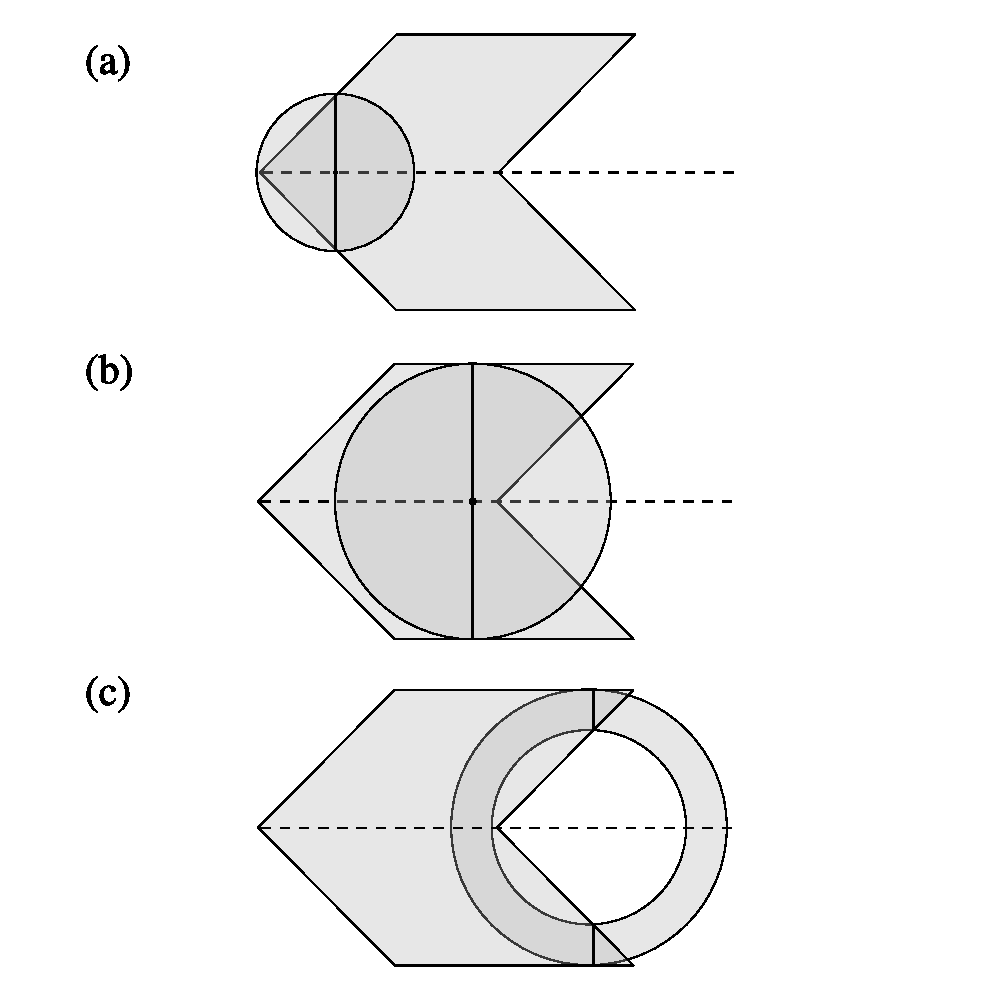
\includegraphics[width=0.5\textwidth]{growingsphere.pdf}
%   \caption{Schematic representation of the growing communicating
%   sphere, over the space--time diagrams, where time is represented on
%   the horizontal direction, and space is represented in the vertical
%   direction.  In (a) the sphere is
%   growing as the surface of first contact has not reached the maximum
%   distance.  In (b) it has reached the maximum distance, so that it
%   remains at the same size.  After a Doomsday event, the signals can
%   still be observed, but the surface of last contact grows }
%   \label{F_growing_sphere}
%\end{figure}
%
%  
%\begin{figure}
%   \centering
%   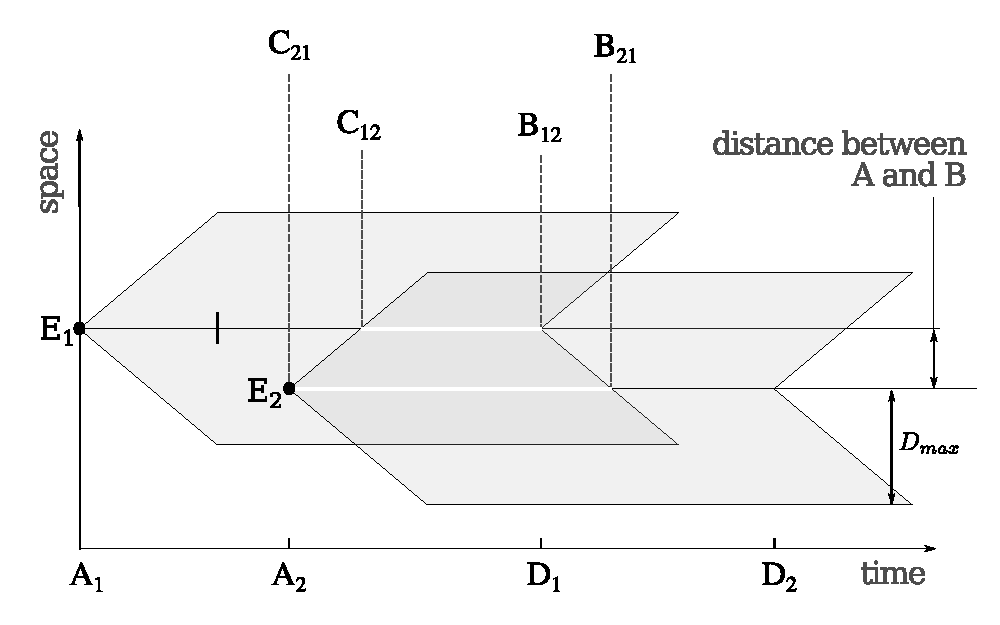
\includegraphics[width=0.5\textwidth]{abcd.pdf}
%   \caption{Schematic representation of two emitters, $E_1$ and $E_2$,
%   that reach each other at different times.  The time span for $E_i$
%   is $(A_i, D_i)$, for $i=\{1,2\}$.  Emitter $i$ can listen to
%   emitter $j$ between $C_{ij}$ and $B_{ij}$.
%   The type and length of causal contact in both directions depend on
%   the distance and time lag between the awakening events, the maximum
%   distance that a signal can reach and the time period in which each
%   emitter is active.}
%   \label{F_abcd}
%\end{figure}

% Schematic representation of the growing communicating
%   sphere, over the space--time diagrams, where time is represented on
%   the horizontal direction, and space is represented in the vertical
%   direction.  In (a) the sphere is
%   growing as the surface of first contact has not reached the maximum
%   distance.  In (b) it has reached the maximum distance, so that it
%   remains at the same size.  After a Doomsday event, the signals can
%   still be observed, but the surface of last contact grows.
%   %
%   Schematic representation of two emitters, $E_1$ and $E_2$,
%   that reach each other at different times.  The time span for $E_i$
%   is $(A_i, D_i)$, for $i=\{1,2\}$.  Emitter $i$ can listen to
%   emitter $j$ between $C_{ij}$ and $B_{ij}$.
%   The type and length of causal contact in both directions depend on
%   the distance and time lag between the awakening events, the maximum
%   distance that a signal can reach and the time period in which each
%   emitter is active.
%
%
%
%   \begin{figure}
%      %
%      \centering
%      %
%      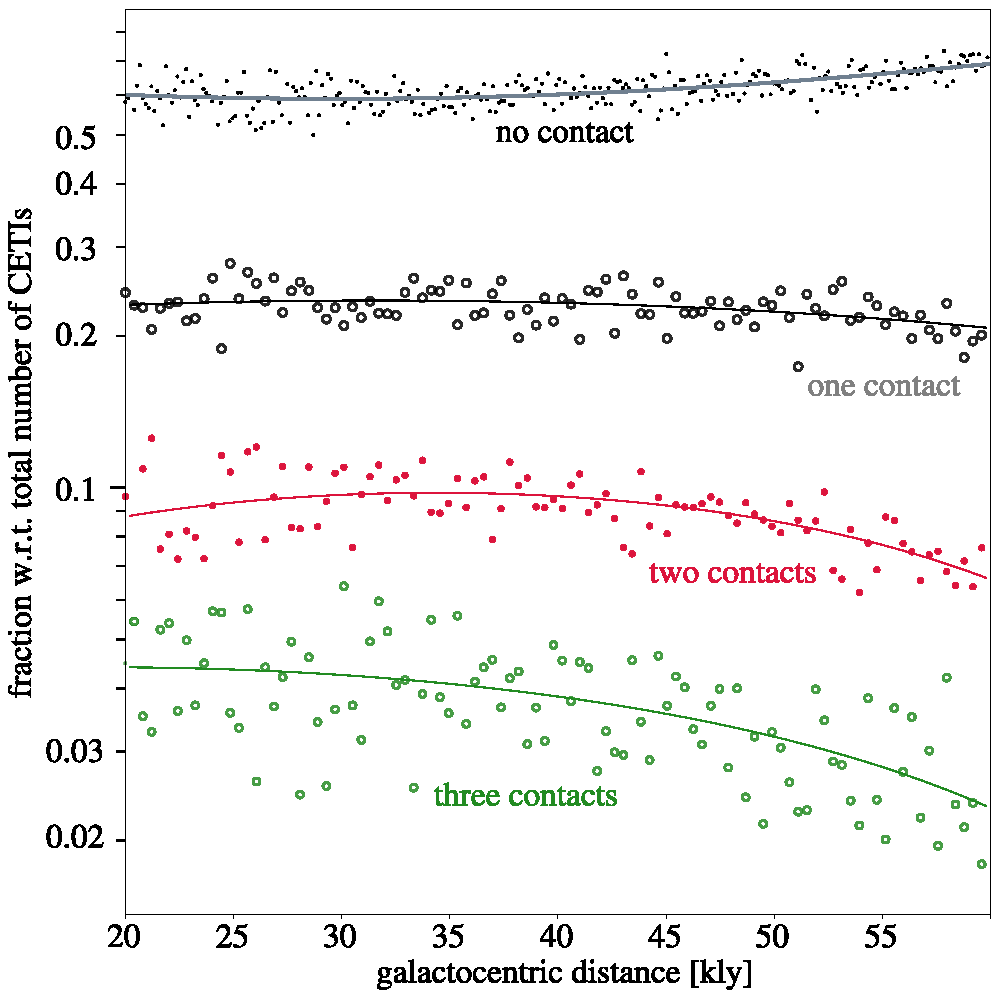
\includegraphics[width=0.45\textwidth]{galactocentric_frac.pdf}
%      %
%      \caption{Fraction of MPLs making cero, one, two or three contacts
%      as a function of galactocentric distance.}
%      %
%      \label{F_radial_frac}
%      %
%   \end{figure}
%}}} 


